\chapter{(Beispielkapitel) Robotersysteme}

Das folgende Kapitel soll als Beispielkapitel dienen. Nach der Kapitelüberschrift wird der Kapitelinhalt in ein paar Sätzen beschrieben.
Hier steht weiterer Text.

\section{PR2}

Der PR2 (Willow Garage Inc., Menlo Park, USA) ist ein \textbf{\textit{menschenähnlicher}} Serviceroboter, der seinen Dienst in Wohnräumen verrichten soll und derzeit im sogenannten PR2 Beta-Programm von elf Forschungseinrichtungen über einen Zeitraum von zwei Jahren getestet wird 
\cite{WillowGarage2010}.
Hier steht weiterer Text.  d

\begin{figure}[!ht]
	\centering
	\subfigure[]{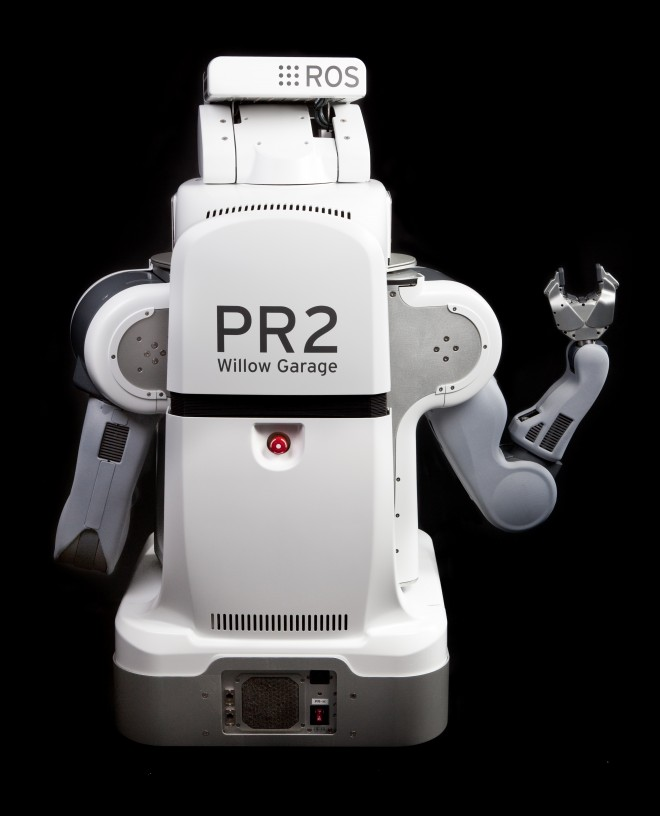
\includegraphics[height=50mm]{PR2-1}}
	\hspace{5mm}
	\subfigure[]{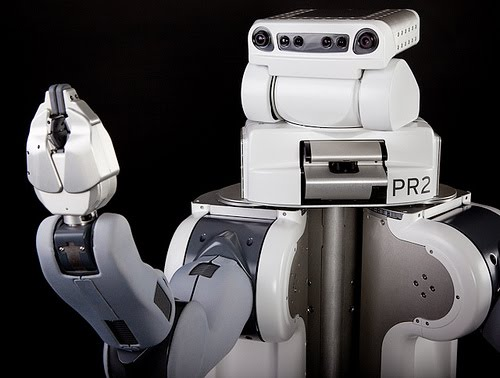
\includegraphics[height=50mm]{PR2-2}}
	\hspace{5mm}
	\subfigure[]{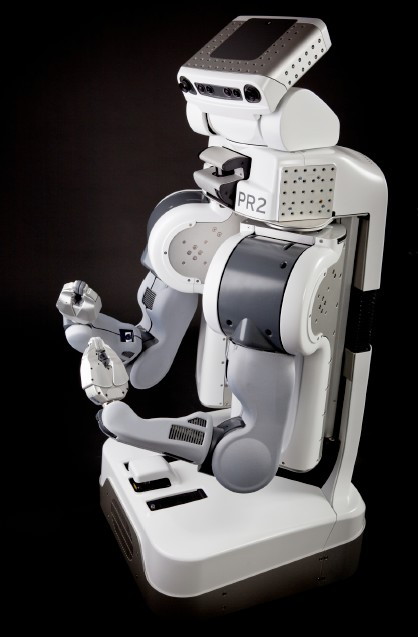
\includegraphics[height=50mm]{PR2-3}}
	\caption{Serviceroboter PR2 von Willow Garage (Quelle: Willow Garage))}
	\label{fig.PR2}
\end{figure}

Ausgestattet ist der PR2 mit zwei Armen, die jeweils sieben Freiheitsgrade haben und an deren Enden ein Greifer montiert ist, siehe \bild{PR2}. Die Sensorik des Armes besteht aus einer Kamera am Unterarm und Druck- sowie Beschleunigungssensoren am Greifer. Die Nutzlast eines Arms ist mit \SI{1,8}{kg} ausgewiesen. Weiterhin verfügt der Roboter über einen dreh- und schwenkbaren Kopf, in dem eine 5-Megapixel Farbkamera, ein LED-Texturprojektor und zwei Stereokameras integriert sind, wobei eine Kamera für die Fernsicht und die andere für die Objektmanipulation genutzt wird. Unterhalb des Kopfes ist ein schwenkbarer Laserscanner und ein Inertialsensor verbaut. Die Position des Oberkörpers lässt sich in der Höhe zwischen \SI{1330}{mm} und \SI{1645}{mm} (Gesamthöhe) variieren. Angetrieben wird die omnidirektionale Basis von vier gelenkten Rädern, die eine maximale Geschwindigkeit von \SI{3,6}{\kilo\metre\per\hour} ermöglichen. Die quadratische Basis hat eine Kantenlänge von \SI{668}{mm}. Als Recheneinheit stehen zwei Server zur Verfügung, die jeweils auf acht CPU-Kernen rechnen und dabei auf 24\,GB Arbeitsspeicher zugreifen können. Als Betriebssystem wird Ubuntu verwendet, auf dem das Robot Operating System, kurz ROS, die Grundlage für die Datenverarbeitung bildet. Da ROS innerhalb dieser Arbeit ebenfalls zum Einsatz kommt, wird dieses in \Sec{ROS} vorgestellt und an den entsprechenden Stellen weiter erläutert. Die Kosten für einen PR2-Roboter belaufen sich derzeit auf etwa \SI{400 000}{\text{US-Dollar}}\footnotemark. Mit Hilfe des PR2 wurden von den zuvor erwähnten Beta-Testern Szenarien bewältigt, die innerhalb des menschlichen Wohnraumes auftreten können. An der TU München hat ein PR2-Roboter beispielsweise zusammen mit einem anderen Robotersystem einen Pfannkuchen gebacken \cite{TUM2011}.
\footnotetext{Der angegebene Preis wurde am 16.08.2011 der Website http://www.willowgarage.com/pages/pr2/order entnommen und versteht sich exklusive Steuern und Versandkosten.}

\section{ROS}
\label{sec.ROS}

Hier steht weiterer Text.

\begin{table}
	\centering
	\caption{Technische Daten der youBot Plattform}\label{tab.TechSpecYouBotBase}
	\vspace*{-3mm}
	\begin{tabular}{lcr}
        \toprule
		Bezeichnung		& Formelzeichen	&              \\
		\midrule
		Gesamtlänge 	& $a$           & \SI{530}{mm} \\
		\rowcolor{Snow2}
		Gesamtbreite 	& $b$           & \SI{350}{mm} \\
		Höhe			& $h$           & \SI{106}{mm} \\
		Radstand		& $l$           & \SI{470}{mm} \\
		\bottomrule
	\end{tabular} 
\end{table}

\begin{lstlisting}[label=source.launchHokuyo,caption=Launchfile zum Start der hokuyo\_node]
<!-- launch hokuyo node -->
<node pkg="hokuyo_node" type="hokuyo_node" name="hokuyo_node" output="screen">
	<param name="port" value="/dev/ttyACM0"/>
	<param name="frame_id" value="/base_laser_front_link"/>
</node>
\end{lstlisting}